\begin{figure}[H]
    \centering
    \subfloat[\footnotesize Accury \textit{w.r.t.} the ratio of data used in unknown class]{
        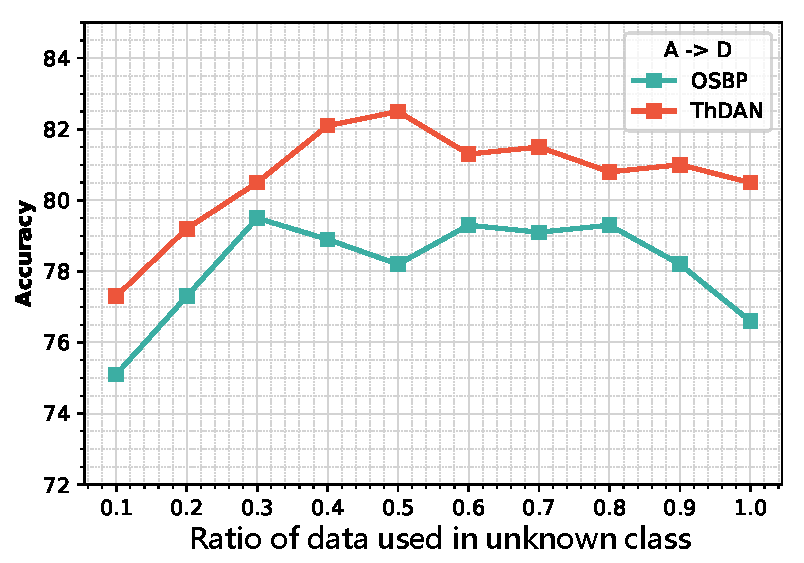
\includegraphics[width=0.3\textwidth]{contents/figures/pdf/analysis/nuknown_change.pdf} 
        \label{figure: ration of unknown}
    } 
    \hspace{2mm}
    \subfloat[\footnotesize Accury \textit{w.r.t.} the number of classes that are treated as the unknown]{
        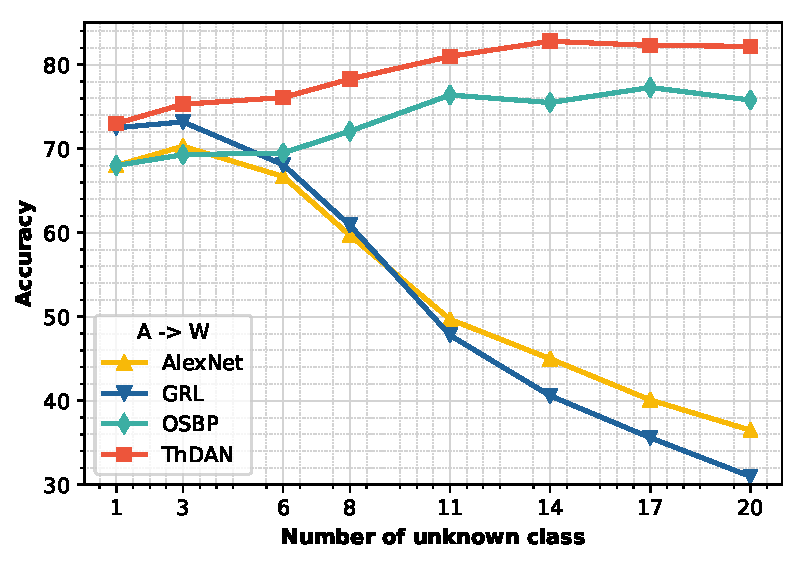
\includegraphics[width=0.3\textwidth]{contents/figures/pdf/analysis/class_change.pdf} 
        \label{figure: number of unknown class}
    }
    \hspace{2mm}
    \subfloat[Accury \textit{w.r.t.} the value of $\gamma_0$]{
        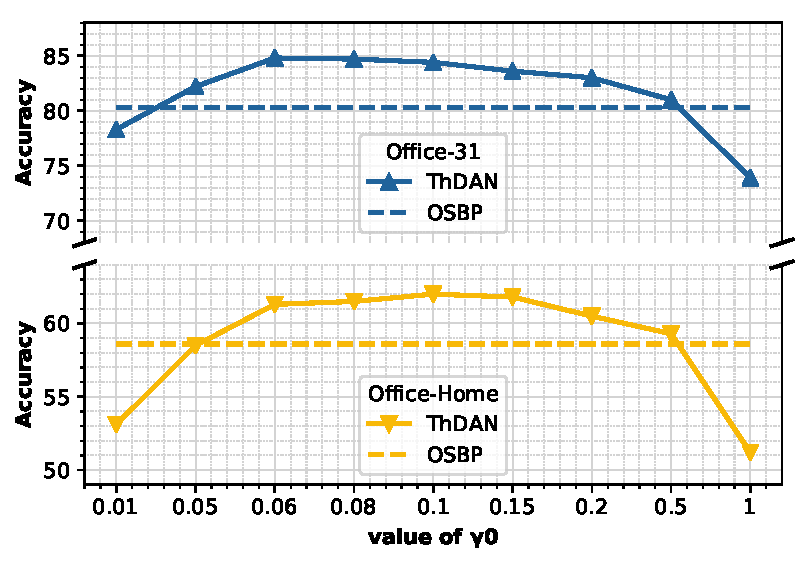
\includegraphics[width=0.3\textwidth]{contents/figures/pdf/analysis/sigma_change.pdf} 
        \label{figure: changing of sigma}
    }
    \\
    \caption{ }
    \label{figure: analysis}
\end{figure}